\section{Entrepôts de données}\label{sec:rw:supervision:warehouse}
Pour l'informatique décisionnelle (\textit{Business Intelligence}), l'approche par entrepôt de données (\textit{Data Warehouses}) est très largement répandue. Son apport est originellement utilisé dans les applications pour entreprises. Toutefois, sa capacité de traitement et ses outils d'analyses ont permis son introduction dans d'autres cœurs de métiers tels que les réseaux~\cite{Gilbert:quicksand} ou l'agriculture~\cite{Abdullah:olap}. Cette architecture est prévue comme support à des outils d'analyses de données puissants. Pour cela, des procédés ont été développés pour faire de l'intégration de données hétérogènes, ainsi que des structures d'entrepôts prêts à répondre aux besoins d'analyses.

Son utilisation dans le cadre de l'observation semble claire. En effet, puisque l'observation et la compréhension du système passent par son analyse, des outils sont nécessaires pour effectuer ces opérations. L'établissement de diagnostic nécessite effectivement le parcours des données pour mieux comprendre les causes d'un problème. De plus, sa structure permettant l'intégration de donnée est à considérer pour intégrer les sources de données hétérogènes auxquelles nous devons faire face.

Par la suite, cette section détaille en premier lieu l'architecture globale de la solution. Nous détaillons ensuite comment l'intégration est faite via les processus \textit{ETL}. Ensuite nous décrivons les structures de données utilisées pour permettre différentes analyses. Enfin, nous présentons brièvement quelques outils d'analyses pouvant raisonner sur les données.

\subsection{Architecture globale}
La définition fonctionnelle d'un entrepôt de donnée est \enquote{\it une collection de données orientées sujet, intégrées, non volatiles et historisées, organisées pour le support d’un processus d’aide à la décision}~\cite{Inmon:warehouse}. Au sens large, un entrepôt est une base de données avec une organisation qui s'oriente avant tout sur l'application finale (l'analyse) plutôt que sur l'intégrité des données, et qui néglige la suppression ou la modification de données afin de garder une trace.
\begin{figure}[ht]
	\centering
	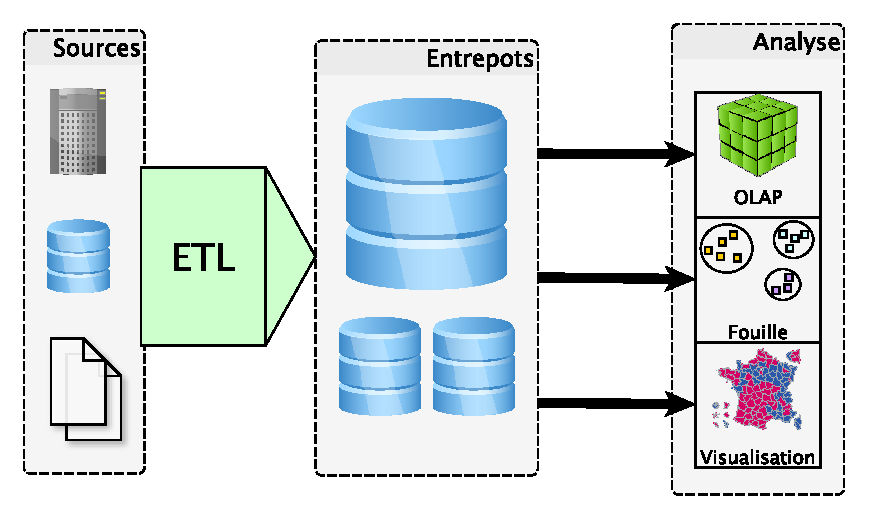
\includegraphics[width=0.65\textwidth]{rw-supervision-warehouses}
	\caption{Architecture globale d'une solution d'entrepôts de données}\label{fig:rw:supervision:warehouses}
\end{figure}
La figure~\ref{fig:rw:supervision:warehouses} présente une architecture abstraite des approches à entrepôts pour intégrer des sources hétérogènes. Afin d'effectuer l'intégration des données à l'intérieur d'un (ou des) entrepôt(s), il est nécessaire de traiter cette hétérogénéité et charger les données. Les processus \textit{ETL} ont été conçus pour cette tâche. Ces procédés sont découpés en trois phases : l'extraction (\textit{\textbf{E}xtract}), le traitement (\textit{\textbf{T}ransform}) et enfin le chargement (\textit{\textbf{L}oad}). Cet aspect est détaillé en section~\ref{sec:rw:supervision:warehouse:etl}.

Par la suite, des outils d'analyses tels que \textit{OLAP}~\cite{Codd:olap} ou d'autres algorithmes de \textit{fouilles de données} sont utilisés pour aider l'utilisateur à prendre une décision. Ainsi, les entrepôts adoptent des modélisations permettant ce type d'analyses telles que les schémas relationnels en étoile ou en flocons~\cite{Levene:snowflake} pour représenter des données multidimensionnelles~\cite{Gray:cube}.

\subsection{L'intégration par ETL}\label{sec:rw:supervision:warehouse:etl}
Afin de charger les données provenant de sources hétérogènes dans un entrepôt, les données sont d'abord extraites des sources. Cette extraction peut être faite par des bases de données intermédiaires. Puis elles sont transformés grâce à une composition d'opérateurs variés~\cite{Vassiliadis:taxonomy}. Enfin, les données sont chargées dans l'entrepôt.

\subsubsection{Chargement}
Plusieurs considérations de performances rentrent en compte pour savoir quand la publication est effective. En effet, lors d'une mise à jour de base de données relationnelle, le système transactionnel requiert que les données soient à jour à la fin de la transaction. Ici, l'écriture effective peut-être retardée pour permettre un chargement des données moins coûteux~\cite{Petit:historical}.

De plus, à cette étape, il est courant de générer des rapports compilant les données transformées vers un document qui est transmis à l'utilisateur.

\subsubsection{Le temps réel : un nouveau challenge}
La fraicheur des données à l'intérieur d'un entrepôt de donnée n'a pas été une contrainte critique jusqu'à présent. Les latences usuellement visées par ce type d'approche sont au alentour de l'heure voire de jours~\cite{Oracle:realtimedw}. Récemment, des travaux se sont intéressés à améliorer la qualité du traitement en terme de fraicheur de données (pour passer à l'ordre de la minute voire de la seconde).

Comme présentée en section~\ref{sec:intro:problematique}, la gestion de l'évolution des données est importante dans notre cadre. Ici, la gestion du dynamisme n'est pas explicite, car il n'y a pas de mécanisme d'événement. Ainsi, il est nécessaire d'implémenter un \textit{CDC} (\textit{Change Data Capture}) capable de transmettre les nouvelles données via un canal de communication dédiée.

Plusieurs systèmes commencent à supporter la gestion en temps réel de l'import de données~\cite{Thomsen:rite, Oracle:ODI}. Toutefois, il n'y a pas de résultats concrets concernant le traitement des données dynamiques en tant que tel. Par exemple, la définition d'agrégat sur une fenêtre de temps doit se faire à la main via une base de données intermédiaire.

\subsection{Synthèse}
En conclusion, les entrepôts de données représentent une grande capacité de traitement des données. La prise en charge de données historique et les capacités d'analyses sont précieuses pour l'observation de système. Toutefois, le processus d'intégration est trop lent pour pouvoir gérer des alertes. De plus, il existe une ambiguïté sémantique sur les opérateurs disponibles qui dépendent du système.

\begin{table}[!ht]
\criteretabDonnee
    {Modèle relationnel}
    {Géré par le modèle relationnel. Modélisation en étoile et par normalisation.}
    {Faible gestion du dynamisme en dehors des mécanismes CDC dans les entrepôts temps réels.}
\criteretabTraitement
    {Instantané principalement. Les ETL peuvent être apparentés à des interrogations continues.}
    {Intégration complexe via les ETL.}
    {Paradigme déclaratif pour l'exploration de données. Algorithmique pour la fouille de données. Principalement procédural pour les ETL.}
    {En dehors des algorithmes et des procédures de gestion de syntaxe ou de règles métiers, le traitement des données est dérivé de l'algèbre relationnelle.}
\criteretabAdaptabilite
    {Spécification du schéma de l'entrepôt. Description des processus ETL. Si les besoins d'analyses sont poussés, il est nécessaire de concevoir les outils d'analyse aussi.}
    {La gestion de données multidimensionnelles apporte cette gestion de perspective de façon native. Il est possible de créer différents sous-entrepôts pour chacun des métiers avec des données agrégées (alimentés par ETL).}
    {Il est très souvent nécessaire de rajouter des opérateurs, ou des logiciels d'analyses plus poussés. Les implémentations permettent en général de rajouter des procédures personnalisées à tous les niveaux de la chaîne.}
    {Les procédés sont lourds et complexes et la durée de réactivité peut se compter en minutes ou en heures. Toutefois, ces systèmes manipulent des Tera de données.}
\caption{Synthèse des entrepôts de données}\label{tab:rw:supervision:warehouses:synthese}
\end{table}